\begin{figure}[h]
    \centering    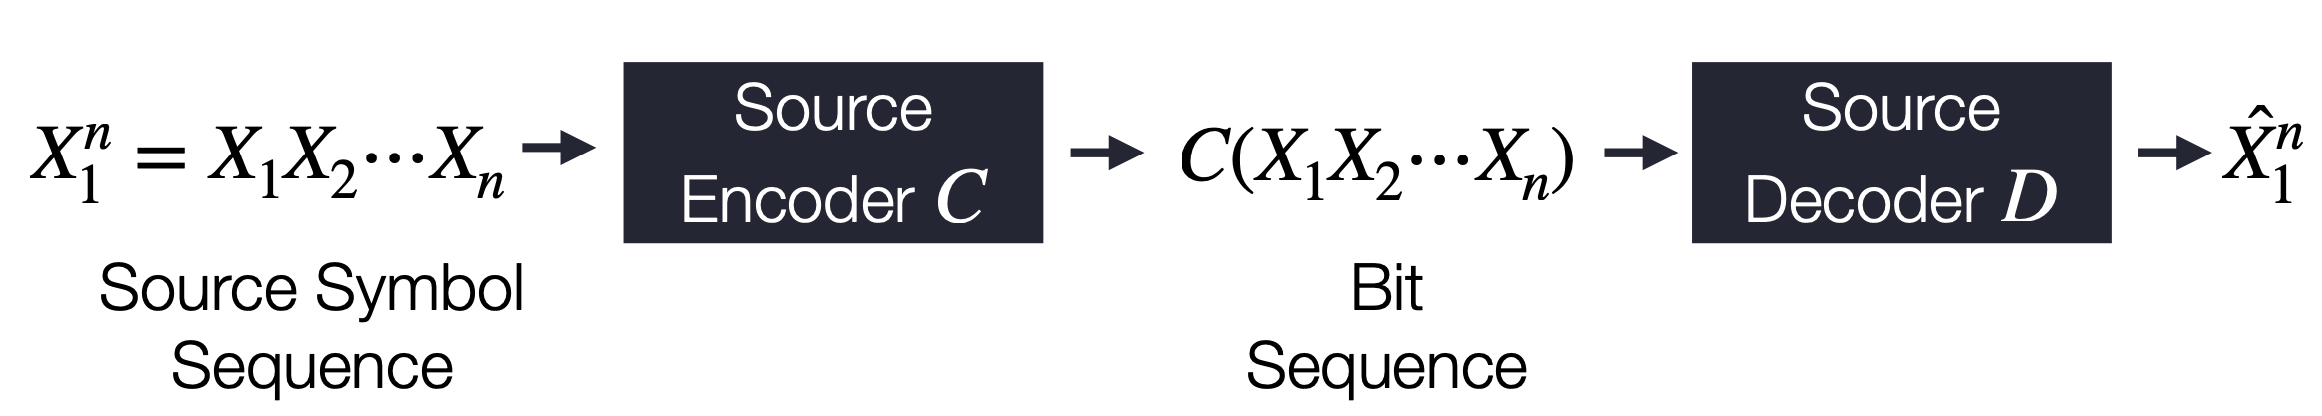
\includegraphics[width=0.75\textwidth]{../images/scribe3-SC.png}
    \caption{Source coding}
\end{figure}
In lossless compression, our objective is to encode a sequence of symbols into a binary string without error, \textit{using as few bits per symbol as possible}.

\subsection{Variable-Length Codes and the Encoding Rate}
Consider a text such as
\[
\texttt{my name is albert}.
\]
Each character (including spaces) is modeled as an outcome of a random variable. An encoder assigns each symbol $x\in\mathcal{X}$ a binary codeword $f(x)\in\{0,1\}^*$. The encoded sequence is then the concatenation
\[
f(x_1)f(x_2)f(x_3)\dots.
\]
The \emph{rate} (average number of bits per symbol) is defined as
\[
\text{Rate} = \mathbb{E}[\ell(x)] = \sum_{x\in\mathcal{X}} p_X(x)\, \ell(x),
\]
where $\ell(x)=|f(x)|$ is the length of the codeword for $x$. Our goal is to minimize this rate.

\subsection{Uniquely Decodable and Prefix-Free Codes}
A code is \emph{uniquely decodable} if every encoded binary sequence corresponds to exactly one original symbol sequence. A special and useful class is that of \emph{prefix-free} codes, where no codeword is a prefix of another. This property ensures that the code can be decoded in linear time.

\paragraph{Example 1 (Uniquely Decodable Code):}  
Let $\mathcal{X}=\{\text{A},\text{B},\text{C}\}$ with the assignment
\[
f(\text{A})=0,\quad f(\text{B})=10,\quad f(\text{C})=11.
\]
The sequence ``ABAC'' is encoded as ``010011''. Since the code is prefix-free, decoding can proceed unambiguously.

\paragraph{Example 2 (Non-Uniquely Decodable Code):}  
Let $\mathcal{X}=\{\text{A},\text{B},\text{C}\}$ with the assignment
\[
f(\text{A})=0,\quad f(\text{B})=1,\quad f(\text{C})=10.
\]
The sequence ``ABAC'' encodes to ``01010'', which is ambiguous as it can be parsed in multiple ways.

\begin{figure}[h]
    \centering
    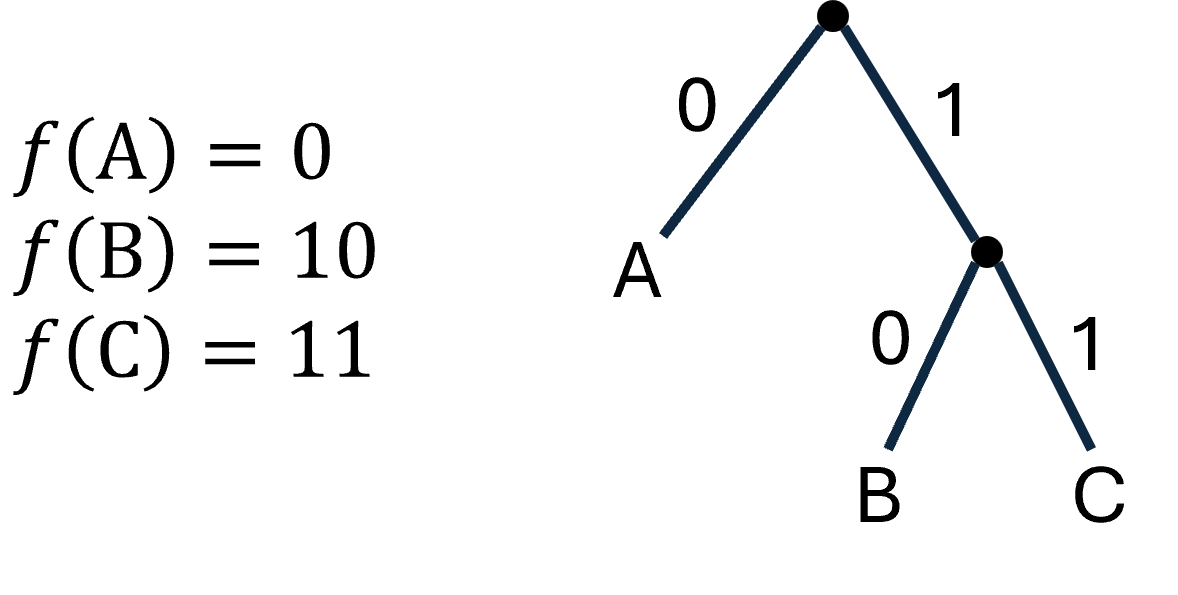
\includegraphics[width=0.4\textwidth]{images/prefixcode_example.png}
    \caption{A prefix-free code represented as a binary tree.}
    \label{fig:prefix_tree}
\end{figure}

\subsection{Optimal Prefix-Free Codes and the Entropy Bound}
For a given source distribution $P_X$, a natural choice is to assign codeword lengths
\[
\ell(x)=\lceil \log \frac{1}{p_X(x)} \rceil.
\]
Then the expected rate is given by
\[
\text{Rate} = \sum_{x}p_X(x)\,\ell(x),
\]
and one can prove the following bound.

\begin{theorem}[Entropy Bound]
For any prefix-free code with codeword lengths $\ell(x)=\lceil \log\frac{1}{p_X(x)} \rceil$, the expected rate satisfies
\[
H(X) \le \text{Rate} < H(X) + 1.
\]
\end{theorem}
\begin{proof}
Since by definition,
\[
\text{Rate} = \sum_{x} p_X(x)\, \lceil \log\frac{1}{p_X(x)} \rceil,
\]
and using the property of the ceiling function
\[
\lceil y \rceil < y + 1 \quad \text{for any } y\in\mathbb{R},
\]
we have for each $x$:
\[
\lceil \log\frac{1}{p_X(x)} \rceil < \log\frac{1}{p_X(x)} + 1.
\]
Taking expectation over $x$, we obtain
\[
\text{Rate} < \sum_{x} p_X(x)\left(\log\frac{1}{p_X(x)}+1\right)
= H(X) + \sum_{x} p_X(x) = H(X) + 1.
\]
On the other hand, since $\lceil y \rceil \ge y$, it follows that
\[
\text{Rate} \ge \sum_{x} p_X(x)\log\frac{1}{p_X(x)} = H(X).
\]
Thus, 
\[
H(X) \le \text{Rate} < H(X) + 1.
\]
\end{proof}

\paragraph{Example 3 (Uniform Distribution):}  
If $\mathcal{X}=\{a,b,c,d\}$ with $p_X(x)=1/4$ for all $x$, then one optimal assignment is
\[
a:00,\quad b:01,\quad c:10,\quad d:11,
\]
achieving a rate of exactly $2$ bits per symbol, which equals $H(X)$.

\paragraph{Example 4 (Non-Uniform Dyadic Distribution):}  
For $\mathcal{X}=\{a,b,c,d\}$ with
\[
p_X(a)=\frac{1}{2},\quad p_X(b)=\frac{1}{4},\quad p_X(c)=p_X(d)=\frac{1}{8},
\]
an optimal code is given by
\[
a:0,\quad b:10,\quad c:110,\quad d:111.
\]
The expected rate is
\[
\text{Rate}= \frac{1}{2}\cdot 1 + \frac{1}{4}\cdot 2 + \frac{1}{8}\cdot 3 + \frac{1}{8}\cdot 3 = 1.75 \text{ bits/symbol},
\]
which is nearly equal to $H(X)=1.75$ bits.

\subsection{Kraft and Kraft-McMillan Inequalities}
\begin{theorem}[Kraft Inequality] For $\mathcal{X}=\{1,2,...,n\}$, 
A set of codeword lengths $\{l(x): x\in\mathcal{X}\}$ corresponds to a prefix-free binary code if and only if
\[
\sum_{x\in\mathcal{X}} 2^{-l(x)} \leq 1.
\]
\end{theorem}
\begin{proof}
Suppose that $l_1 \leq l_2 \leq \cdots \leq l_n$. Let $A$ be a full binary tree of depth $l_n$. Each word of length $l_i$ corresponds to a node $v_i$ in this tree at length $l_i$. The subtree $A_i$ of $A$ rooted at $v_i$ has $2^{l_n-l_i}$ elements. And by the prefix-free property, $A_i\cap A_j=\emptyset\text{ for }i\neq j.$  Thus, $$
\Biggl|\bigcup_{i=1}^nA_i\Biggr| =\sum_{i=1}^n2^{l_n-l_i}\leq2^{l_n}=|A|.
$$

Conversely, set of codeword lengths $\{l_i\,:\,i=1,...,n\}$ satisfying this inequality, one can construct a prefix-free code by a greedy procedure.
\end{proof}

The Kraft-McMillan inequality extends this result to any uniquely decodable code:
\[
\sum_{x\in\mathcal{X}} 2^{-l(x)} \leq 1.
\]

\begin{proof}
Denote $T=\sum_{i=1}^n2^{-l_i}.$ The idea of the proof is to get an upper bound on $T^n$ and show that it can only hold for all $n\in\mathbb{N}$ if $T \leq 1$.
Rewrite $T^n$ as
$$
\begin{aligned}
    T^n = \left(\sum_{i=1}^n 2^{-l_i}\right)^n=\sum_{i_1=1}^n\sum_{i_2=1}^n\cdots\sum_{i_n=1}^n2^{-(l_{i_1}+l_{i_2}+\cdots +l_{i_n})}.
\end{aligned}
$$
Consider $\mathcal{X}^n$. Since $\mathcal{X}$ was assumed to uniquely decodable, we can rewrite the equation to
$$T^n = \sum_{l=1}^{n\cdot l_{\max}} A_l 2^{-l}$$,
where $A_l$ corresponds to number of $l$-length words. Since $A_l\leq 2^{l}$, we can finally obtain
$$T^n = \sum_{l=1}^{n\cdot l_{\max}} A_l 2^{-l}\leq n\cdot l_{\max} \implies T=\sum_{i=1}^n 2^{-l_i}\leq (n \cdot l_{\max})^{\frac{1}{n}}$$. The right-hand side is $1$ asymptotically.
\end{proof}
Moreover, any uniquely decodable code can be transformed into a prefix-free code without altering the codeword lengths.

\subsection{Cost of Mismatch in Compression}
When the true source distribution is $P_X$ but an estimated distribution $Q$ is used to design the code, the codeword lengths are assigned as
\[
l(x)=\log\frac{1}{q(x)}.
\]
Then, the expected length under the true distribution is
\[
\mathbb{E}_{P_X}[l(x)] = \sum_{x} p_X(x)\log\frac{1}{q_X(x)}.
\]
We can decompose this as
\[
\mathbb{E}_{P_X}[l(x)] = \sum_{x} p_X(x)\log\frac{p_X(x)}{q(x)} + \sum_{x} p_X(x)\log\frac{1}{p_X(x)} = D(P_X\|Q) + H(X).
\]
Thus, the additional cost due to the mismatch is exactly the KL divergence $D(P_X\|Q)$.

\subsection{Huffman Codes}
Huffman coding is an algorithm that produces an optimal prefix-free code for a given source distribution.

\subsubsection*{Huffman Algorithm}
\begin{enumerate}
    \item Identify the two symbols with the smallest probabilities.
    \item Merge these two symbols into a composite symbol whose probability is the sum of the two.
    \item Repeat the process on the reduced set of symbols until only one symbol remains, thereby forming a binary tree.
\end{enumerate}

\subsubsection*{Optimality Conditions}
Huffman codes satisfy the following conditions:
\begin{itemize}
    \item If $p(x_1) > p(x_2)$, then the optimal code must have $\ell(x_1) \le \ell(x_2)$.
    \item The two least probable symbols $a_{M-1}$ and $a_M$ receive codewords of equal length.
\end{itemize}

\begin{proof}(Sketch for condition 1)
Assume, to the contrary, that there exist symbols $x_1$ and $x_2$ with $p(x_1) > p(x_2)$ but $\ell(x_1) > \ell(x_2)$. By swapping the codewords of $x_1$ and $x_2$, the overall expected codeword length decreases, which contradicts the assumption of optimality.\\\\
(Sketch for condition 2) Suppose $l_M > l_{M-1}$. We can immediately find a better code since the code has a binary tree representation.
\end{proof}

\begin{figure}[h]
    \centering
    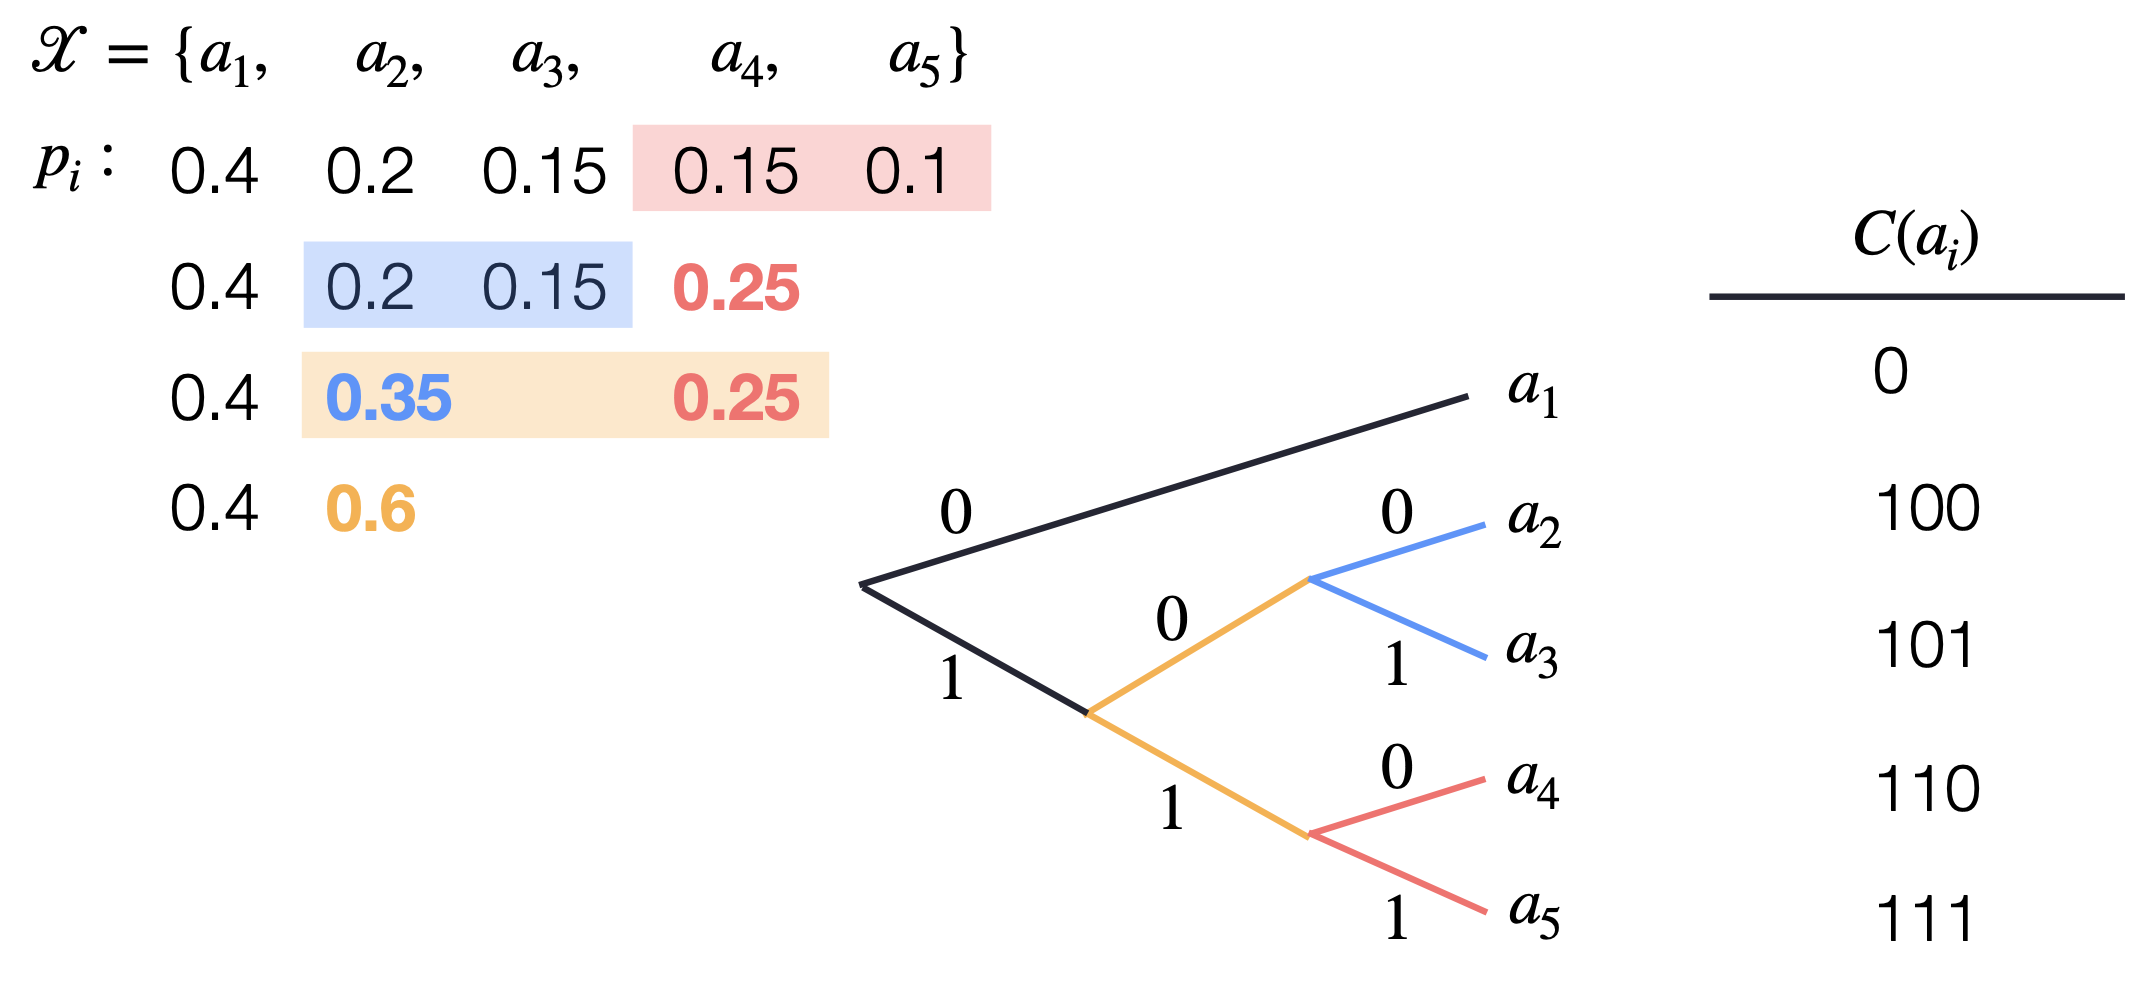
\includegraphics[width=0.7\textwidth]{images/Huffman.png}
    \caption{Example of a Huffman coding tree.}
    \label{fig:huffman_example}
\end{figure}

Although Huffman coding minimizes the expected codeword length among symbol-by-symbol prefix-free codes, we have
\[
H(X) \le \mathbb{E}[\ell(X)] < H(X) + 1,
\]
with the gap due to the integer constraint on the codeword lengths. This gap can be reduced by encoding blocks of symbols.

\subsection{Asymptotic Equipartition Property (AEP)}
The AEP underpins block coding approaches by demonstrating that, as the block length grows, almost all sequences are \emph{typical}.

\begin{definition}[$\epsilon$-Typical Sequence]
For a discrete source $X$ with distribution $P_X$, a sequence $x^n$ is called \emph{$\epsilon$-typical} if
\[
\left|-\frac{1}{n}\log p_X(x^n)-H(X)\right|\le \epsilon
\]
or equivalently, 
\[
2^{-n(H(X)+\epsilon)}\leq p_X(x^n) \leq 2^{-n(H(X)-\epsilon)}
\]
Let $A_{\epsilon}^{(n)}$ denote the set of all $\epsilon$-typical sequences, called the typical set.
\end{definition}

\begin{theorem}[AEP]
For any $\epsilon > 0$,
\[
\lim_{n\to\infty} \text{Pr}\{x^n\in A_{\epsilon}^{(n)}\} = 1.
\]
\end{theorem}
\begin{proof}
\[
\begin{aligned}
\text{Pr}\{X^n \in A^n\} 
&= \text{Pr}\left\{ \left| -\frac{1}{n}\log p_X(X^n) - H \right| \leq \epsilon \right\} \\
&= 1 - \text{Pr}\left\{ \left| -\frac{1}{n}\log p_X(X^n) - H \right| > \epsilon \right\} \\
&\stackrel{(1)}{=} - \text{Pr}\left\{ \left|\frac{1}{n}\sum_{i=1}^{n}\log\frac{1}{p_X(X_i)} - H\right| > \epsilon \right\} \\
&\stackrel{(2)}{\geq} 1 - \frac{\sigma^2}{n\epsilon^2} \\
&\to 1 \text{ as } n \to \infty
\end{aligned}
\]
(1) by iid, (2) by Markov inequality.
\end{proof}

\begin{theorem}[Size of Typical Set]
The size of the $\epsilon$-typical set satisfies:
\[
(1-\epsilon)2^{n(H(X)-\epsilon)} \le |A_{\epsilon}^{(n)}| \le 2^{n(H(X)+\epsilon)}.
\]
\end{theorem}
\begin{proof}
\text{The upper bound:}
\[
1 \geq \text{Pr}\left\{X^n \in A_{\epsilon}^{(n)}\right\}
= \sum_{x^n \in A_{\epsilon}^{(n)}} p_X(x^n)
\geq \sum_{x^n \in A_{\epsilon}^{(n)}} 2^{-n(H(X) + \epsilon)}
= \left|A_{\epsilon}^{(n)}\right| 2^{-n(H(X) + \epsilon)},
\]
which gives the upper bound. For the lower bound, by the AEP, for any \(\epsilon > 0\), there exists sufficiently large \(n\) such that

\[
1 - \epsilon \leq \text{Pr}\left\{X^n \in A_{\epsilon}^{(n)}\right\}
= \sum_{x^n \in A_{\epsilon}^{(n)}} p_X(x^n)
\leq \sum_{x^n \in A_{\epsilon}^{(n)}} 2^{-n(H(X) - \epsilon)}
= \left|A_{\epsilon}^{(n)}\right| 2^{-n(H(X) - \epsilon)}.
\]
\end{proof}

\subsection{Near-Lossless Compression}
Block coding allows us to approach the entropy limit arbitrarily closely.

\begin{theorem}[Achievability]
For any rate $R>H(X)+\epsilon$, there exists a compression scheme that maps the typical set $A_{\epsilon}^{(n)}$ into binary strings of length $\lceil nR\rceil$, ensuring that the probability of decoding error tends to zero as $n\to\infty$.
\end{theorem}
\begin{proof}
Fix $R > H(X) + \delta$. For $n$ sufficiently large, by the theorem 16 and 17, 
$$
\text{Pr}\left\{X^n \notin A_\delta^{(n)}\right\} < \epsilon
$$
and
$$
\left|A_\delta^{(n)}\right| \leq2^{n(H(X)+\delta)}=2^{nR}.
$$
Consider a scheme that enumerates sequences in $A_{\delta}^{(n)}$. The encoder maps $X^n \in A_\epsilon^{(n)}$ to its binary representation. Otherwise, it outputs $(0,0,\,...,\,0)$. The decoder maps this binary representation back to the corresponding sequence in $A_\delta^{(n)}.$ Thus, the error probability is bounded by
$$
P_e \leq \text{Pr}\left\{X^n \notin A_\delta^{(n)}\right\} < \epsilon
$$
and the rate is equal to
$$
\frac{\log \left|A_\delta^{(n)}\right|}{n} \leq \frac{nR}{n}=R.
$$
Thus, $R$ is an achievable rate.
\end{proof}

\begin{theorem}[Converse]
Any compression scheme with rate $R<H(X)$ cannot achieve near-lossless recovery as $n\to\infty$.
\end{theorem}
\begin{proof}
For $\delta > 0$, suppose $R < H(X)-\delta$. The size of possible output is $2^{nR}.$ Let $B$ denote the set of (uniquely decodable) reconstruction sequences $\hat{X}^n$. Then 
$$
\begin{aligned}
    \text{Pr}\left\{X^n \in B^c\right\} &\geq \text{Pr}\left\{X^n \in B^c \cap A_\delta^{(n)}\right\}\\
    &=\sum_{x^n\in B^c \cap A_\delta^{(n)}}p(x^n)\\
    &\geq \left|B^c \cap A_\delta^{(n)}\right|\cdot2^{-n(H(X)+\delta)}\\
    &\geq \left(|A_\delta^{(n)}|-\left|B\right|\right)\cdot2^{-n(H(X)+\delta)}\\
    & \approx (2^{nH(X)}-2^{nR})\cdot2^{-nH(X)}\\ &=1-2^{n(R-H(X))} \rightarrow 1 \text{ as } n\rightarrow \infty
\end{aligned}
$$
\end{proof}

\subsection{Arithmetic Encoding}

In contrast to Huffman coding (which suffers from exponential complexity in block-length), arithmetic encoding efficiently represents sequences by mapping them to a subinterval of \([0,1)\).

Arithmetic encoding assigns a sequence \( x^n=(x_1,x_2,\ldots,x_n) \) an interval \([L,H)\) whose length equals the probability of the sequence:
\[
H - L = p(x^n) = p_X(x_1)\, p_X(x_2\,|\, x_1) \cdots p_X(x_n\,|\, x_1^{n-1}).
\]
Initially, the interval is \([0,1)\). This interval is recursively subdivided into subintervals according to the probabilities of the symbols in the alphabet. For example, if the alphabet is \(\{A, B, C\}\) with probabilities \(p_X(A)=p_A\), \(p_X(B)=p_B\), \(p_X(C)=p_C\), then the interval is partitioned proportionally to these probabilities.

\paragraph{Example (Encoding “AB”):}  
Suppose the first symbol \(A\) maps to the interval \([0,0.25)\) and \(B\) maps to \([0.25,0.4)\) (according to their probabilities). Then, the string “AB” is encoded as the interval \([0.25,0.4)\). Choose 
\[
Z = \frac{L+H}{2} = 0.325,
\]
whose binary expansion is approximately
\[
0.325 \approx 0.0101001100\ldots_{(2)}.
\]

\subsection{Truncation and Decoding}

Since the binary expansion of \(Z\) may be infinite, we choose to truncate it. Write
\[
Z = 0.Z_1Z_2\cdots Z_K\cdots, \quad \hat{Z} = 0.Z_1Z_2\cdots Z_K.
\]
We select the smallest integer \(K\) such that
\[
L \le \hat{Z} < \hat{Z} + 2^{-K} < H.
\]
This condition guarantees that the truncated value \(\hat{Z}\) still uniquely identifies a number within the interval \([L,H)\).

\paragraph{Example (Truncation for “AB”):}  
For the interval \([0.25,0.4)\) and \(Z=0.325\), if \(K=2\) then \(\hat{Z} = 0.01_{(2)} = 0.25\); however, \(\hat{Z} + 2^{-2} = 0.25+0.25 = 0.5\) is not contained in \([0.25,0.4)\). With \(K=3\), \(\hat{Z} = 0.010_{(2)} = 0.25\) and \(\hat{Z} + 2^{-3} = 0.25+0.125=0.375\), which lies in \([0.25,0.4)\). Hence, \(K=3\) is sufficient.

Decoding proceeds by using the received truncated binary number \(\hat{Z}\) to reconstruct the interval partitioning—that is, the decoder repeats the subdivision process to identify the original sequence \(x^n\).

\subsection{Properties and Optimality of Arithmetic Encoding}
Let us prove the key property of arithmetic encoding.

\begin{theorem}[Property of Arithmetic Encoding]
Let \(Z \in [L,H)\) be represented by a truncated binary expansion using \(k\) bits such that
\[
L \le \hat{Z} < \hat{Z} + 2^{-k} < H.
\]
Then,
\[
2^{-k} \ge \frac{1}{4}(H-L).
\]
\end{theorem}
\begin{proof}
Assume the truncated value is 
\[
\hat{Z} = 0.x_1x_2\cdots x_k,
\]
and let \(\tilde{Z}\) denote the truncation to \(k-1\) bits:
\[
\tilde{Z} = 0.x_1x_2\cdots x_{k-1}.
\]
By the minimality of \(k\) (i.e., \(k\) is chosen as the smallest integer for which the condition holds), one of the following must occur:
\[
\tilde{Z} < L \quad \text{or} \quad \tilde{Z} + 2^{-(k-1)} > H.
\]
Suppose, without loss of generality, that
\[
\tilde{Z} < L.
\]
Then, since the condition fails for \(k-1\) bits, we must have 
\[
\tilde{Z} + 2^{-(k-1)} > \frac{L+H}{2}.
\]
Rearranging yields
\[
2^{-(k-1)} > \frac{H-L}{2},
\]
which implies
\[
2^{-k} \ge \frac{1}{4}(H-L).
\]
A similar argument holds if \(\tilde{Z} + 2^{-(k-1)} > H\).
\end{proof}

Using this inequality, one can show that if a sequence \(x^n\) is encoded by arithmetic encoding, then the codeword length \(\ell(x^n)\) satisfies
\[
\ell(x^n) \le \log \frac{1}{p(x^n)} + 2.
\]
Hence, the average length obeys
\[
\mathbb{E}[\ell(X^n)] \le H(X^n) + 2.
\]
Dividing by \(n\), the rate satisfies
\[
R \le H(X) + \frac{2}{n},
\]
so that for large \(n\) the rate approaches the entropy—demonstrating near-optimality.

\subsection{Conditional Entropy}
Before discussing sources with memory, we recall the definition of conditional entropy and its key properties.

\begin{definition}[Conditional Entropy]
For two random variables \(X\) and \(Y\) with joint distribution \(p_{X,Y}(x,y)\), the conditional entropy of \(X\) given \(Y\) is defined as
\[
H(X \,|\, Y) = \sum_{y} p_Y(y) \, H(X \,|\, Y=y),
\]
where
\[
H(X \,|\, Y=y) = \sum_{x} p_{X\,|\, Y}(x \,|\, y) \log \frac{1}{p_{X\,|\, Y}(x \,|\, y)}.
\]
\end{definition}

\begin{remark}
Conditional entropy quantifies the average uncertainty remaining about \(X\) once \(Y\) is known.
\end{remark}

Important properties include:
\begin{itemize}
    \item \textbf{Chain Rule:} For any pair of random variables,
    \[
    H(X,Y) = H(Y) + H(X \,|\, Y).
    \]
    More generally, for a sequence \(X_1, X_2, \ldots, X_n\),
    \[
    H(X_1, X_2, \ldots, X_n) = H(X_1) + \sum_{i=2}^{n} H(X_i \,|\, X_1, \ldots, X_{i-1}).
    \]
    \item \textbf{Functional Dependence:} \(H(X \,|\, Y) = 0 \iff X=g(Y)\) almost surely.
    \item \textbf{Reduction of Uncertainty:} \(H(X \,|\, Y) \le H(X)\), with equality if and only if \(X\) and \(Y\) are independent.
\end{itemize}

\subsection{Sources with Memory: Markov Processes}

Thus far we assumed that the input sequence is i.i.d.; however, practical sources (e.g., text) are highly correlated. A common model for such dependencies is the Markov process.

\subsubsection{First-Order Markov Process}
\begin{definition}
A sequence \(X_1, X_2, \dots, X_n\) is said to follow a \emph{first-order Markov process} if
\[
p_X(x_i\,|\, x_1,x_2,\dots,x_{i-1}) = p_X(x_i\,|\, x_{i-1})
\]
for all \(i \ge 2\).
\end{definition}
Then, the joint distribution factors as
\[
p(x^n) = p_X(x_1) \prod_{i=2}^{n} p_X(x_i \,|\, x_{i-1}),
\]
and the joint entropy is
\[
H(X^n) = H(X_1) + \sum_{i=2}^{n} H(X_i \,|\, X_{i-1}).
\]
If the chain is \emph{stationary} (i.e., the marginal distribution of each \(X_i\) is the same), then
\[
H(X^n) = H(X_1) + (n-1)H(X_2 \,|\, X_1),
\]
so that the fundamental limit per symbol is
\[
\lim_{n \to \infty} \frac{1}{n} H(X^n) = H(X_2 \,|\, X_1).
\]

\paragraph{Example (Random Walk):}  
Consider the random walk defined by
\[
X_0 = 0,\quad X_n = X_{n-1} \pm 1 \quad \text{with probability } \frac{1}{2} \text{ each}.
\]
This process is Markov (i.e., the future depends only on the present). (Note: A simple random walk is not stationary since its variance grows with \(n\); here the example serves to illustrate the Markov property.)

\subsubsection{\(k\)th-Order Markov Process}
\begin{definition}
A sequence \(X_1, X_2, \dots, X_n\) follows a \emph{\(k\)th-order Markov process} if
\[
p_X(x_i\,|\, x_1,\dots,x_{i-1}) = p_X(x_i\,|\, x_{i-k},\dots,x_{i-1})
\]
for all \(i > k\).
\end{definition}
Then,
\[
p(x^n) = \left[\prod_{i=1}^{k} p_X(x_i)\right] \prod_{i=k+1}^{n} p_X(x_i \,|\, x_{i-k}^{i-1}),
\]
and the fundamental limit becomes
\[
\lim_{n \to \infty}\frac{1}{n}H(X^n) = H(X_{k+1}\,|\, X_1^k).
\]

\subsubsection{Stationary Distribution and Entropy Rate}
\begin{definition}[Entropy Rate]
For a stationary process \(\{X_i\}_{i=1}^{\infty}\), the \emph{entropy rate} is defined as
\[
H(\mathscr{X}) = \lim_{n\to\infty} \frac{1}{n} H(X_1,X_2,\dots,X_n).
\]
\end{definition}
For the i.i.d. case, \(H(\mathscr{X})=H(X)\); for a stationary first-order Markov process,
\[
H(\mathscr{X})=H(X_2\,|\, X_1);
\]
and for a stationary \(k\)th-order Markov process,
\[
H(\mathscr{X})=H(X_{k+1}\,|\, X^k).
\]

\paragraph{Example (Stationary First-Order Markov):}  
Assume a process over three symbols \(\{A,B,C\}\) with an initial uniform distribution, i.e., \( p_X(A)=p_X(B)=p_X(C)=\frac{1}{3} \), and transition probabilities
\[
p_X(x_2\,|\, x_1) = \frac{1}{3} \quad \text{for all } x_1,x_2.
\]
Then the process is stationary and
\[
H(\mathscr{X}) = H(X_2\,|\, X_1) = \log 3.
\]

\begin{figure}[htpb]
\begin{center}
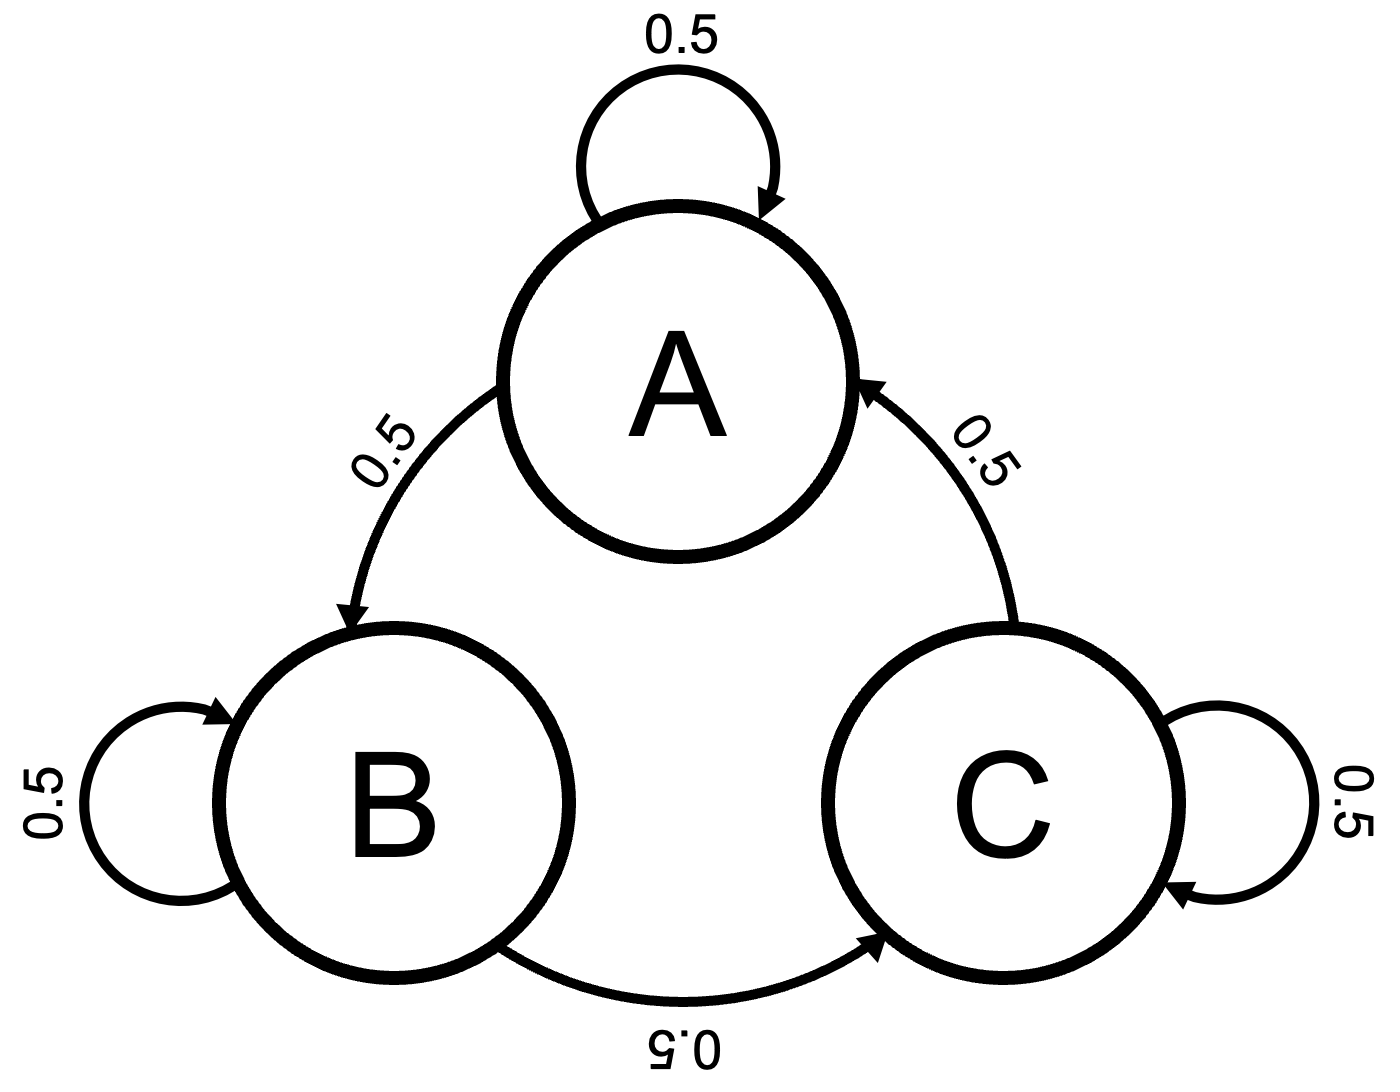
\includegraphics[scale=0.3]{images/scribe12-markovex.png}
\caption{\(1^\text{st}\) order Markov transition example.}
\label{fig:markovtrans}
\end{center}
\end{figure}

\paragraph{Example(Achievability of the Fundamental Limit):}
Consider a stationary first-order Markov source \(X_1,X_2,\ldots,X_n\). By the Markov property,
\[
p(x^n)=p_X(x_1)\prod_{i=2}^{n} p_X(x_i\,|\, x_{i-1}).
\]
Arithmetic encoding maps \(x^n\) to an interval of length
\[
H - L = p(x^n).
\]
Then, as shown earlier, the expected codeword length satisfies
\[
\mathbb{E}[\ell(X^n)] \le \log\frac{1}{p(x^n)} + 2.
\]
Taking the expectation and normalizing by \(n\), and under the stationarity assumption, we obtain
\[
R \leq \frac{1}{n}\left( H(X_1) + 2 \right) + \frac{n-1}{n}H(X_2\,|\, X_1).
\]
Letting \(n\to\infty\) yields
\[
R \approx H(X_2\,|\, X_1) = H(\mathscr{X}),
\]
establishing the achievability of the fundamental limit. A similar derivation holds for stationary \(k\)th-order Markov sources, for which the limit is \( H(\mathscr{X})=H(X_{k+1}\,|\, X^k) \).

\begin{remark}
In these notes we restrict our attention to stationary sources. The fundamental limit as given by the entropy rate holds only under stationarity.
\end{remark}


\subsection{Unknown Source Distribution and Universal Compression}
\label{sec:unknown_source}

Assume \(X_1, \dots, X_m\) are i.i.d.\ random variables with \(X_i \sim P_X\), but the true distribution \(P_X\) is unknown. One universal compression scheme is to use the first \(m\) symbols both to learn the distribution and to “synchronize” the encoder and decoder, and then to compress the remaining \(X_{m+1},\dots,X_n\) using a code designed from the estimated distribution.

A simple scheme is as follows:
\begin{enumerate}
    \item Examine (and encode) \(X_1,\dots,X_m\) using a pre-agreed, fixed (sub-optimal) code.
    \item Use these \(m\) symbols to compute an empirical estimate \(\hat{P}_X\) of the true distribution \(P_X\).
    \item Both encoder and decoder construct a Huffman code (or another optimal prefix-free code) based on \(\hat{P}_X\).
    \item Compress the remaining sequence \(X_{m+1},\dots,X_n\) using the newly constructed code.
\end{enumerate}

There is an inherent trade-off in the choice of \(m\): a larger \(m\) improves the accuracy of \(\hat{P}_X\) (and thus the compression rate may approach \(H(X)\)), but more bits are wasted to transmit the first \(m\) symbols using the fixed code. Conversely, a smaller \(m\) reduces the learning overhead but may yield a poor estimate of \(P_X\).

\subsection{Lempel-Ziv Algorithms}
\label{sec:lz}
Unlike the scheme above, which separates the learning and execution phases, Lempel-Ziv algorithms perform both simultaneously.

\subsubsection*{LZ78 Algorithm}
The LZ78 algorithm parses an input sequence into variable-length phrases while dynamically building a dictionary. The parsing rule is:
\begin{enumerate}
    \item Initialize the dictionary to be empty.
    \item Starting at the beginning of the sequence, find the longest prefix \(w\) that is already in the dictionary.
    \item Output the tuple \((d, a)\), where \(d\) is the index of \(w\) in the dictionary (or 0 if \(w\) is empty) and \(a\) is the next symbol that extends \(w\) (thus \(w a\) is the new phrase).
    \item Add \(w a\) to the dictionary.
    \item Continue parsing from the symbol following \(w a\).
\end{enumerate}

\paragraph{Example.}  
Consider a sequence over the alphabet \(\{A, B\}\):
\[
\texttt{ABBABABAAABB}\ldots
\]
The parsing (with dictionary updates) proceeds as follows:
\begin{itemize}
    \item \textbf{Step 1:} The dictionary is initially empty. The first symbol \(A\) is not in the dictionary. Output \((0, A)\) and add \(A\) as phrase 1.
    \item \textbf{Step 2:} Next, consider \(B\). It is new, so output \((0, B)\) and add \(B\) as phrase 2.
    \item \textbf{Step 3:} The next symbols are \(B\). The algorithm finds that \(B\) is already in the dictionary (as phrase 2). Now, check the extension: after \(B\) comes \(A\) (i.e. the string “BA” is not in the dictionary). Output \((2, A)\) and add “BA” as phrase 3.
    \item \textbf{Step 4:} Continue with the next unparsed symbol. The sequence now starts with \(B\). \(B\) is in the dictionary. Check the extension: \(B\) followed by \(A\) gives “BA,” which is in the dictionary (phrase 3); then extend further: “BA” followed by \(B\) is “BAB,” which is new. Output \((3, B)\) and add “BAB” as phrase 4.
    \item \textbf{Step 5:} Next, the remaining portion begins with \(A\). Since \(A\) is already in the dictionary, check extension. If “A” followed by \(A\) (i.e. “AA”) is not in the dictionary, output \((1, A)\) and add “AA” as phrase 5.
    \item \textbf{Step 6:} Continue in this fashion for the rest of the input.
\end{itemize}

Each phrase is then encoded using an efficient binary representation of its tuple. Over time, frequently occurring phrases lead to long dictionary entries.

\begin{figure}[h]
    \centering
    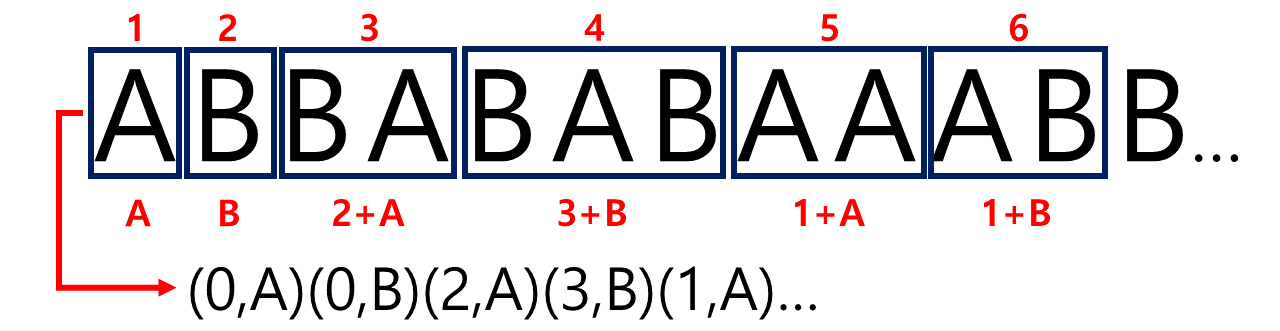
\includegraphics[width=0.8\textwidth]{images/scribe14_figure.png}
    \caption{Mapping input symbols into a sequence of tuples (phrases) in LZ78.}
    \label{fig:lz78}
\end{figure}

Lempel-Ziv algorithms, like LZ78, are universal, meaning they asymptotically achieve the entropy rate \(H(\mathscr{X})\) for any stationary source \(\mathbb{X}\) without prior knowledge of \(P_X\).


\subsection{Mutual Information and Conditional Mutual Information}

\subsubsection{Mutual Information}
Mutual information between two random variables \( X \) and \( Y \) measures the reduction in uncertainty about one random variable due to knowledge of the other. Formally, mutual information is defined as:
\[
I(X;Y) = H(X) - H(X|Y) = H(Y) - H(Y|X).
\]

Mutual information is symmetric and can also be expressed in terms of KL divergence:
\[
I(X;Y) = D(p_{X,Y}\,\|\,p_X p_Y) = \sum_{x,y} p_{X,Y}(x,y)\log\frac{p_{X,Y}(x,y)}{p_X(x)p_Y(y)}.
\]

Mutual information satisfies the following important properties:

\begin{itemize}
    \item \textbf{Symmetry:} 
    \[
    I(X;Y) = I(Y;X).
    \]

    \item \textbf{Non-negativity:} 
    \[
    I(X;Y)\ge 0.
    \]
    Equality holds if and only if \(X\) and \(Y\) are independent.

    \item \textbf{Self-Information:} 
    \[
    I(X;X) = H(X).
    \]
\end{itemize}

\paragraph{Example.} If \(X\) and \(Y\) are independent, then 
\[
I(X;Y)=H(X)-H(X\,|\,Y)=H(X)-H(X)=0.
\]

\subsubsection{Conditional Mutual Information}

Conditional mutual information quantifies how much knowing one random variable reduces uncertainty about another, given that a third variable is already known:
\[
I(X;Z\,|\,Y)=H(X\,|\,Y)-H(X\,|\,Y,Z).
\]

Conditional mutual information satisfies similar properties to mutual information:

\begin{itemize}
    \item \textbf{Non-negativity:}
    \[
    I(X;Z\,|\,Y)\geq 0.
    \]
    Equality holds if and only if \(X\) and \(Z\) are conditionally independent given \(Y\).

    \item \textbf{Chain Rule:} 
    \[
    I(X^n;Y)=\sum_{i=1}^{n}I(X_i;Y\,|\,X^{i-1}).
    \]
    \item If \(X\) and \(Z\) are independent but become dependent when conditioned on \(Y\), then:
    \[
    I(X;Z)=0\quad\text{but}\quad I(X;Z\,|\,Y)>0.
    \]

    \item Conversely, if \(X\to Y\to Z\) is Markov, then:
    \[
    I(X;Z\,|\,Y)=0\quad\text{but potentially}\quad I(X;Z)>0.
    \]
\end{itemize}

\paragraph{Example} Suppose:
\[
X,Z\sim\text{Bernoulli}(1/2)\quad\text{and}\quad Y=X\oplus Z.
\]

Then:
\[
I(X;Z)=0,\quad\text{but}\quad I(X;Z\,|\,Y)=1,
\]

showing explicitly how conditioning can increase mutual information.

\subsubsection{Data Processing Inequality}


A fundamental property of mutual information is the \emph{data processing inequality} (DPI), which intuitively says that processing data cannot increase its information content about the original source. 

\begin{theorem}[Data Processing Inequality]
If random variables \(X\), \(Y\), and \(Z\) form a Markov chain \(X\to Y\to Z\), then
\[
I(X;Z)\leq I(X;Y).
\]
\end{theorem}

\begin{proof}
Since \(X\to Y\to Z\) is a Markov chain, it implies that given \(Y\), \(Z\) is conditionally independent of \(X\):
\[
p_{Z\,|\,X,Y}(z\,|\,x,y) = p_{Z\,|\,Y}(z\,|\,y).
\]

Then, by the chain rule for mutual information:
\[
I(X;Y,Z) = I(X;Y) + I(X;Z\,|\,Y).
\]

But due to the Markov chain, \(I(X;Z\,|\,Y)=0\), thus:
\[
I(X;Y,Z) = I(X;Y).
\]

Since adding information (i.e., considering \(Y,Z\) jointly) cannot decrease mutual information, we have:
\[
I(X;Z) \leq I(X;Y,Z) = I(X;Y).
\]
\end{proof}

\noindent\textbf{Interpretation:} The data processing inequality states that no data processing can increase the information content about an original source.

\noindent\textbf{Remark:}
\begin{itemize}
    \item If $X\to Y \to Z$, then $Z \to Y \to X$.
    \item If $Z=g(Y)$, then $X \to Y \to Z$.
    \item If $X\to Y \to Z$, then $I(X;Z\,|\,Y)=0$.
\end{itemize}
